\documentclass{article}

\usepackage[utf8]{inputenc}
\usepackage[T1]{fontenc}
\usepackage[francais]{babel}
\usepackage{amssymb}
\usepackage{amsmath}
\usepackage{amsthm}
\usepackage{graphics}
\usepackage{enumerate}

\newtheorem{proposition}{Proposition}
\newtheorem{definition}{Définition}
\newtheorem{theoreme}{Théorème}
\newtheorem{lemme}{Lemme}


\begin{document}

\title{Courbe elliptique et théorème de Mordell-Weil}
\date \today
\author{Duhamel Nicolas}
\maketitle


L'objectif de ce TER est de donner une introduction aux courbes elliptiques et de démontrer un cas
particulier du théorème de Mordell-Weil qui énonce que les points rationnels d'une courbe elliptique
forment un groupe abélien engendré par un nombre fini de points.

On commencera par des "rappels" de géométrie projective, qui est le cadre naturel des courbes elliptiques,
même si il est généralement plus commode de travailler dans le plan affine en ajoutant un point à l'infini.
On donnera ensuite une définition des courbes elliptiques et démontrerons un cas particulier du
théorème de Mordell-Weil.
Par ailleurs, nous verrons en cours de route que toute courbe elliptique peut être représenter par
une équation simple dite équation de Weierstrass.
Finalement, on présentera une approche des courbes elliptiques par l'analyse complexe à partir des
fonctions elliptiques qui sont des fonctions avec deux périodes indépendantes, cette partie nous permettra
de démontrer l'associativité de la loi de groupe sur la courbe elliptique.

La grande majorité du contenu du TER est tiré de \cite{silverman_rational_1992} qui donne une introduction au
théorème de Mordell-Weil, pour des livres plus généraux sur les courbes elliptiques voir
\cite{cassels_lectures_1991} et \cite{mckean_elliptic_1999}.

\section{Géométrie projective}
On se contentera de présenter le plan projectif et les courbes dans le plan projectif, ce qui sera
tout ce dont nous auront besoin dans la suite.
\subsection{Le plan projectif}
Le plan projectif $\mathbb{P}_{2}(K)$ est l'ensemble des triplets $[a,b,c]$ avec $a,b,c$ non tous nuls
muni de la relation d'équivalence $[a,b,c] \sim [a',b',c']$ si et seulement si il existe 
$t\in K^{*}$ tel que $a=ta', b=tb', c=tc'$. Les nombres $a,b,c$ sont appelés les coordonnées homogènes
du point $[a,b,c]$.

Le plan affine $\mathbb{A}_{2}(K)$ est l'ensemble des points $(x,y)\in K^{2}$. A tout point 
$(x,y)\in \mathbb{A}_{2}(K)$ correspond un point $[x,y,1]=[X,Y,Z] \in \mathbb{P}_{2}(K)$.
Réciproquement, si $Z \neq 0$, tout point $[X,Y,Z]\in \mathbb{P}_{2}(K)$ est associé au point
$(x,y)\in \mathbb{A}_{2}(K)$ oé $x=\frac{X}{Z}$ et $y=\frac{Y}{Z}$.

Voyons maintenant à quoi correspond un point $[X,Y,Z]\in \mathbb{P}_{2}(K)$ avec $Z=0$, pour cela considérons
dans le plan affine deux droites parallèles $L: ax+by+c=0$ et $L': a'x+b'y+c'=0$ oé $a'=ta$, $b'=tb$ et $t\neq 0$.
En coordonnées homogènes, ces droites deviennent $L: aX+bY+cZ=0$ et $L': a'X+b'Y+c'Z=0$, l'intersection de ces
droites a lieu au point $[b, -a, 0] \in \mathbb{P}_{2}(K)$ donc en un point où $Z=0$.
On voit donc que les points $[X,Y,Z]\in \mathbb{P}_{2}(K)$ avec $Z=0$ correspondent aux directions affines,
où une direction est une classe d'équivalence de droites parallèles dans le plan affine.
Cela nous permet de décrire $\mathbb{P}_{2}(K)$ sous la forme
\begin{equation*}
\mathbb{P}_{2}(K) = \mathbb{A}_{2}(K) \cup \{\text{directions de }\mathbb{A}_{2}(K)\}
\end{equation*}

\begin{proposition}
Deux droites projectives distinctes $L: aX+bY+cZ=0$ et $L': a'X+b'Y+c'Z=0$ de $\mathbb{P}_{2}(K)$ ont un unique point d'intersection.
Réciproquement, deux points distincts de $\mathbb{P}_{2}(K)$ définissent une unique droite.
\end{proposition}

\begin{proof}
Pour la première partie distinguons deux cas:
\begin{enumerate}[(i)]
\item $L: ax+by+c=0$ et $L': ax+by+c=0$ se coupent dans le plan affine en $(x_{0}, y_{0})$, alors
L et L' s'intersecte dans le plan projectif en $[x_{0}, y_{0}, 1]$.
\item L et L' sont parallèles dans le plan affine donc $a'=ta$, $b'=tb$ avec $t\neq 0$, alors
L et L' se coupent au point $[b, -a, 0]$
\end{enumerate}

Réciproquement, soit $[X_{1}, Y_{1}, Z_{1}]$ et $[X_{2}, Y_{2}, Z_{2}]$ deux points distincts.
La droite $L: aX+bY+cZ=0$ passent par ces deux points si et seulement si
\begin{equation*}
\left\lbrace
\begin{array}{lcl}
aX_{1}+bY_{1}+cZ_{1} &=& 0\\
aX_{2}+bY_{2}+cZ_{2} &=& 0
\end{array}\right.
\end{equation*}
C'est un système à deux équations indépendantes et 3 inconnues donc un espace de solutions de dimension 1
où toutes ces droites sont identifiées à une seule droite projective.
\end{proof}

On voit donc que le plan projectif nous permet de ne plus faire la distinction entre droites parallèles ou non,
deux droites distinctes se coupent toujours en un unique point quitte à rajouter des points à l'infini.

\subsection{Courbes dans le plan projectif}
On définit une courbe dans le plan projectif comme l'ensemble des solutions d'une équation polynomiale $F(X,Y,Z)=0$.
Un point $[X, Y, Z]\in \mathbb{P}_{2}(K)$ admet plusieurs représentations, le polynôme doit donc vérifier
$F(a,b,c)=0$ si et seulement si $F(ta,tb,tc)=0$ pour $t\neq 0$

Si $F(X,Y,Z)=\sum{a_{ijk}X^{i}Y^{j}Z^{k}}$ est de degré d, 
\begin{equation*}
t^{-d}F(tX, tY, tZ) = \sum_{i+j+k=d}{a_{ijk}X^{i}Y^{j}Z^{k}} + 
\sum_{i+j+k < d}{t^{i+j+k-d}a_{ijk}X^{i}Y^{j}Z^{k}}
\end{equation*}

En un point $[X,Y,Z] \in C$, si F n'est pas homogène de degré d alors quand $t$ tend vers 0, le terme de gauche 
est nul tandis que le terme de droite diverge; contradiction.

Cela nous permet de dire que toute courbe est définie par un polynôme homogène. Si $F$ est un polynôme
homogène de degré d, on dira alors que la courbe $C: F(X,Y,Z)=0$ est de degré d.

On va maintenant faire le lien avec l'identification entre le plan affine 
et le plan projectif privé des points à l'infini.

Si $[a,b,c]\in C$ avec $c\neq 0$, comme $F(a,b,c)=0$ et $F$ est un polynôme homogène de degré d, on obtient que
\begin{equation*}
F(\frac{a}{c}, \frac{b}{c}, 1)=c^{-d}F(a,b,c)=0
\end{equation*}
On définit alors le polynôme $f(x,y)=F(x,y,1)$,
d'après ce qui précède il y a donc une bijection entre $\{[a,b,c]\in C, c\neq 0\}$ et $\{f(x,y)=0\}$.
On dit alors que la courbe $f(x,y)=0$ est la partie affine de la courbe projective $C$.

Ce processus qui consiste à remplacer le polynôme homogène $F(X,Y,Z)$ par un polynôme non-homogène
$f(x,y)=F(x,y,1)$ est appelé déshomogénéisation.

Réciproquement, étant donné une courbe affine $f(x,y)=0$, on transforme $f(x,y)$ en un polynôme homogène $F(X,Y,Z)$ tel que
$F(x,y,1)=f(x,y)$.

Si $f(x,y) = \sum{a_{ij}x^{i}y^{j}}$ est un polynôme de degré d, on définit l'homogénéisation de $f(x,y)$ par
\begin{equation*}
F(X,Y,Z)=\sum{a_{ij}X^{i}Y^{j}Z^{d-i-j}}
\end{equation*}
On peut voir que $F(X,Y,Z)$ est bien un polynôme homogène de degré d et que $F(x,y,1)=f(x,y)$.
On obtient ainsi une correspondance entre les courbes affines et les courbes projectives.

Afin de donner une définition des courbes elliptiques, on aura besoin que la courbe est une tangente
en tout point, c'est à dire que la courbe ne contiennent pas de point singulier.

Un point $[a,b,c]$ d'une courbe projective $C: F(X,Y,Z)=0$ est dit singulier si
\begin{equation*}
\frac{\partial F}{\partial X}(a,b,c) = \frac{\partial F}{\partial Y}(a,b,c) = \frac{\partial F}{\partial Z}(a,b,c) = 0
\end{equation*}
On dira que C est une courbe lisse si tous ses points sont non singuliers. Si $[a,b,c]\in C$ est un point non singulier,
la courbe admet une tangente au point $[a,b,c]$ d'équation
\begin{equation*}
\frac{\partial F}{\partial X}(a,b,c)X + \frac{\partial F}{\partial Y}(a,b,c)Y + \frac{\partial F}{\partial Z}(a,b,c)Z = 0
\end{equation*}

Remarque : Le point $[a,b,c]$ appartient bien à la tangente d'après la formule d'Euler sur les polynômes homogènes.

\section{Courbes elliptiques}

\begin{definition}
Une courbe elliptique est une cubique non singulière qui admet une solution non triviale dans $K$.
On note $E(K) \subset \mathbb{P}_{2}(K)$ l'ensemble des points d'une courbe elliptique sur un corps $K$.
\end{definition}

\subsection{Forme normale de Weierstrass}
Dans la suite, on va montrer qu'en effectuant un changement de coordonnées l'équation de la courbe elliptique devient
\begin{equation*}
V^2W + a_{1}UVW + a_{2}VW^2 = U^3 + a_{3}U^2W + a_{4}UW^2 + a_{5}W^3
\end{equation*}
Si la caractéristique de $K$ est différente de 2 et 3, on effectue le changement de variable
$Y=V + \frac{a_{1}}{2}U + \frac{a_{2}}{2}W$, $X=U+\frac{1}{3}(a_{3}-\frac{a_{1}^2}{4})$ et $Z=W$,
on obtient l'équation sous forme de Weierstrass courte que l'on utilisera dans la suite
\begin{equation}
\label{Weier}
Y^2Z=X^3+aXZ^2+bZ^3
\end{equation}

\begin{proposition}
On note $\Delta = -(4a^3+27b^2)$ le discriminant de l'équation \ref{Weier}.
La courbe définie par l'équation \ref{Weier} est singulière si et seulement si $\Delta = 0$
\end{proposition}

\begin{proof}
Si $P=[X,Y,Z]\in E(K)$ est un point singulier alors
\begin{equation*}
\left\lbrace
\begin{array}{lcl}
3X^2 + aZ^2 &=& 0\\
2YZ &=& 0 \\
Y^2 - 2aXZ - 3bZ^2 &=& 0
\end{array}\right.
\end{equation*}
Si $Z=0$, alors $X=Y=0$ contradiction; on peut donc supposer que $Z=1$. On en déduit que $Y=0$ et 
$X^2 = -\frac{a}{3} = \frac{9b^2}{4a^2}$, donc $\Delta = -(4a^3+27b^2) = 0$.

Réciproquement, si $\Delta = 0$ alors $-\frac{3b}{2a}$ est solution de $X^3+aX+b$. En effet, $-27b^2=4a^3$
on a donc
\begin{align*}
(-\frac{3b}{2a})^3 + a(-\frac{3b}{2a}) + b &=  -\frac{27b^3}{8a^3} -\frac{3b}{2} + b\\
			   &= \frac{b}{2} -\frac{3b}{2} + b = 0
\end{align*}
On en déduit que le point $(-\frac{3b}{2a}, 0, 1) \in E(K)$ est un point singulier.
\end{proof}

Soit $F(X,Y,Z)$ un polynôme homogène de degré $3$ tel que $E: F(X,Y,Z)=0$ définit une courbe elliptique et
$P\in E(K)$. On va commencer par traiter le cas plus simple où $P$ est un point d'inflexion et on fera ensuite
le cas général.

\subsubsection{Point d'inflexion}
On envoie le point $P$ en $O=[0,1,0]$ et la tangente en $P$ sur la droite $Z=0$. Soit $Q\neq P$ un point sur la tangente
en $P$ et $R$ tel que $P,Q$ et $R$ sont linéairement indépendant. On définit alors le changement de coordonnées qui envoie $(P,Q,R)$
en $([0,1,0], [1,0,0], [0,0,1])$, la droite $Z=0$ passe par $[0,1,0]$ et $[1,0,0]$ donc le changement de coordonnées
envoie bien la tangente en $P$ sur la droite $Z=0$. La courbe dans les nouvelles coordonnées a pour équation
\begin{align*}
G(X,Y,Z) = &aY^3 + bY^2Z + cYZ^2 + dX^3 + eXY^2 + fXYZ \\
			& + gXZ^2 + hX^2Y + iX^2Z + jZ^3 = 0
\end{align*}
Or le point $O=[0,1,0]$ est sur la courbe, donc $G([0,1,0])=a=0$. De plus, la tangente en $O$ est la droite $Z=0$
donc $\frac{\partial G}{\partial X}([0,1,0])=e=0$ et $\frac{\partial G}{\partial Z}([0,1,0])=b\neq 0$.
L'intersection entre la courbe et la droite $Z=0$ est
\begin{equation*}
dX^3 + hX^2Y = 0
\end{equation*}
Le point $O=[0,1,0]$ est un point triple donc $h=0$ et $d\neq0$.

L'équation de la courbe est maintenant
\begin{equation*}
G(X,Y,Z) = bY^2Z + cYZ^2 + dX^3 + fXYZ + gXZ^2 + iX^2Z + jZ^3 = 0
\end{equation*}
Quitte à diviser par $d\neq 0$, on peut supposer que $d=1$. Pour obtenir l'équation que l'on cherche on pose
$U=X$, $V=Y$ et $W=-\frac{Z}{b}$. On obtient l'équation de la courbe elliptique sous forme de Weierstrass longue
\begin{equation*}
V^2W + a_{1}UVW + a_{2}VW^2 = U^3 + a_{3}U^2W + a_{4}UW^2 + a_{5}W^3
\end{equation*}

\subsubsection{Cas général}
On suppose maintenant que le point $P$ n'est pas un point d'inflexion, donc la tangente en $P$ coupe la courbe
elliptique en un point $Q\neq P$. Si $Q$ est un point d'inflexion, on applique la partie précédente au point $Q$.
Dans le cas où $Q$ n'est pas un point d'inflexion, on prend la tangente en $Q$ qui coupe la courbe elliptique 
en un point $R\neq Q$. Les points $P, Q$ et $R$ ne sont pas colinéaires, sinon les tangente en $P$ et en $Q$ coïncident
et donc coupent la courbe elliptique avec multiplicité $4$; contradiction. On en déduit que $P, Q$ et $R$ sont trois
point sur la courbe elliptique linéairement indépendant. On considère alors le changement de coordonnés qui envoie
$P, Q$ et $R$ en $[1,0,0], [0,1,0]$ et $[0,0,1]$. La courbe dans les nouvelles coordonnées a pour équation
\begin{align*}
G(X,Y,Z) = &aY^3 + bY^2Z + cYZ^2 + dX^3 + eXY^2 + fXYZ \\
			& + gXZ^2 + hX^2Y + iX^2Z + jZ^3 = 0
\end{align*}
Comme $[1,0,0], [0,1,0]$ et $[0,0,1]$ sont sur la courbe elliptique, on en déduit que $a=d=j=0$. La tangente en
$[1,0,0]$ est la droite $Z=0$ donc $\frac{\partial G}{\partial Y}([1,0,0])=h=0$ et 
$\frac{\partial G}{\partial Z}([1,0,0])=i\neq 0$. De méme la tangente en $[0,1,0]$ est la droite $X=0$ donc
$\frac{\partial G}{\partial Z}([0,1,0])=b=0$ et $\frac{\partial G}{\partial X}([0,1,0])=e\neq 0$

L'équation de la courbe devient alors
\begin{equation*}
cYZ^2 + eXY^2 + fXYZ + gXZ^2 + iX^2Z = 0
\end{equation*}
On pose $[X, Y, Z]=[U^2, VW, UW]$, on a alors
\begin{equation*}
cU^2VW^3 + eU^2V^2W^2 + fU^4VW + gU^4W^2 + iU^5W = 0
\end{equation*}
Le changement de variable est bien défini sauf si $[U, V, W]=[0, 0, 1]$ ou $[0, 1, 0]$.
On cherche à inverser cette transformation, on a
\begin{equation*}
[XZ, XY, Z^2]=U^2W[U, V, W]
\end{equation*}
On en déduit que l'inverse est bien définie sauf si $[X, Y, Z]=[0, 1, 0]$ ou $[1, 0, 0]$.

On reprend l'équation, en divisant par $U^2W$ on obtient
\begin{equation*}
cVW^2 + eV^2W + fU^2V + gU^2W + iU^3 = 0
\end{equation*}
Comme précédemment quitte à diviser par $i\neq 0$ et à remplacer $W$ par $-\frac{W}{e}$ ($e\neq 0$), on obtient
alors la forme de Weierstrass longue pour la courbe elliptique
\begin{equation*}
V^2W + a_{1}UVW + a_{2}VW^2 = U^3 + a_{3}U^2W + a_{4}UW^2 + a_{5}W^3
\end{equation*}

\subsection{Loi de groupe}
On va définir une structure de groupe sur la courbe elliptique
\begin{equation*}
E: y^{2} = f(x) = x^{3} + ax + b
\end{equation*}
dont
l'élément neutre sera le point à l'infini $O=[0,1,0]\in E(K)$.

Pour $P,Q\in E(K)$, on trace la droite passant par $P$ et $Q$, on note $P*Q$ le troisiéme point d'intersection.
Si $P=Q$, on considére la tangente en $P$.
Soit $L: cx+dy+e=0$ la droite passant par $P$ et $Q$, si $L$ n'est pas verticale autrement dit $d\neq 0$, alors
la droite $L$ s'écrit sous la forme
\begin{equation*}
L: y=\frac{-e-cx}{d}=\lambda x + \nu
\end{equation*}
et les points d'intersections de $C$ et $L$ sont les solutions de l'équation
\begin{equation*}
(\lambda x + \nu)^2 = x^3 + ax + b
\end{equation*}
qui admet 3 solutions dont deux correspondent à $P$ et $Q$. La droite et la cubique se coupent en un troisième
point que l'on a noté $P*Q$. Ce point est dans $E(K)$, en effet la somme des racines est à valeurs dans $K$ et les
deux premières racines sont à valeurs dans $K$ par hypothèse donc la dernière aussi.

On définit alors la loi de groupe sur $E(K)$ par la formule suivante
\begin{equation*}
P+Q = O*(P*Q)
\end{equation*}
Voir la figure \ref{loigpe} pour une vision géométrique de la loi de groupe.
Le point $O=[0,1,0]\in E(K)$ étant le point à
l'infini qui correspond à la direction verticale, il faut comprendre $O*P$ comme étant l'autre point
d'intersection entre la droite verticale passant par $P$ et la courbe elliptique; autrement dit $O*(x,y)=(x,-y)$
car la courbe $E$ est symétrique par rapport à l'axe des abscisses.

\begin{figure}[t]
\begin{center}
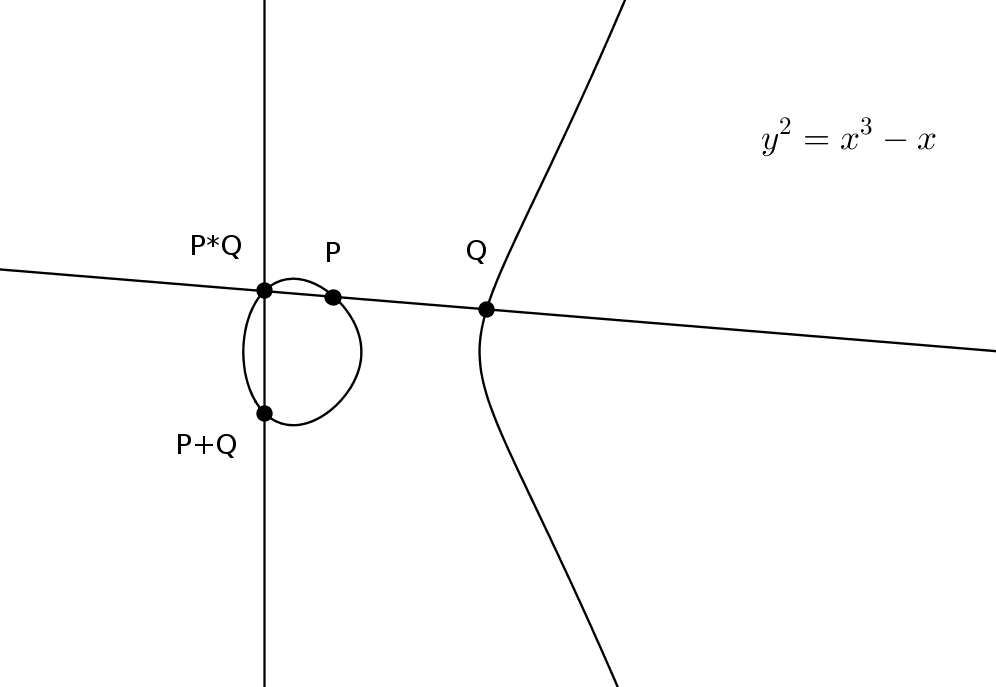
\includegraphics{cub.png}
\end{center}
\caption{Loi de groupe}
\label{loigpe}
\end{figure}

\begin{theoreme}
(E(K), +) est un groupe abélien.
\end{theoreme}

\begin{proof}
On définit l'inverse de P par $-P = P*(O*O)$.

On vérifie que $-P$ est bien l'inverse de $P$,
\begin{equation*}
P + (-P) = O*(P*(P*(O*O))) = O*(O*O) = O
\end{equation*}
Par construction, $P + Q$ et $-P$ sont des points de la courbe $E(K)$.
La définition de $P+Q$ étant symétrique en P et Q, on en déduit immédiatement que
\begin{equation*}
P+Q=Q+P
\end{equation*}
De plus, on vérifie que $O$ est l'élément neutre
\begin{equation*}
O+P=P+O=O*(P*O)=P
\end{equation*}

La seule chose non immédiate est l'associativité, on se reportera à la dernière section pour une
démonstration utilisant les fonctions elliptiques.
\end{proof}

\subsubsection{Formule explicite}
On a vu plus haut que, la coordonnée $x$ du point $P*Q$ est la troisième solution de
$(\lambda x + \nu)^2 = x^3 + ax + b$ qui devient après simplification
\begin{equation*}
x^{3} - \lambda^{2}x^2 + (a-2\lambda \nu)x + b - \nu^2 = 0
\end{equation*}
on en déduit que $x_{1} + x_{2} + x_{3} = \lambda^2$, d'où $x_{3} = \lambda^2 - x_{1} - x_{2}$
et $y_{3} = \lambda x_{3} + \nu$

Il nous reste à expliciter la pente $\lambda$ de la droite pour avoir une formule en fonction
des coordonnées des points $P$ et $Q$.

Si $P\neq \pm Q$, autrement dit $x_{1} \neq x_{2}$, alors
\begin{equation*}
\lambda = \frac{y_{2} - y_{1}}{x_{2} - x_{1}}
\end{equation*}
On en déduit la formule suivante
\begin{equation}
\label{P+Q}
x(P+Q) = (\frac{y_{2} - y_{1}}{x_{2} - x_{1}})^2 - x_{1} - x_{2}
\end{equation}

Si les deux points sont égaux, d'après le théorème des fonctions implicite, 
la pente de la tangente est
\begin{equation*}
\lambda = \frac{dy}{dx} = \frac{f'(x)}{2y}
\end{equation*}
On obtient alors après simplification
\begin{equation}
\label{2P}
x(2P) = \frac{x^4 - 2ax^2 - 8bx + a^2}{4(x^3 + ax + b)}
\end{equation}

\section{théorème de Mordell-Weil}
La démonstration du théorème de Mordell-Weil repose sur un argument de descente, à partir d'un point
sur la courbe elliptique, on va pouvoir faire descendre sa "hauteur" en utilisant un nombre fini d'autre point
de la courbe elliptique jusqu'à tomber dans un ensemble fini.

Pour ce faire, on va définir la hauteur d'un point sur une courbe elliptique et en donner certaines propriétés
générales qui nous permettront de voir que la hauteur diminue bien au cours du processus.

\subsection{Hauteurs}
La hauteur d'un point rationnel mesure d'une certaine manière sa complexité en tant que fraction rationnelle.
Soit $x=\frac{m}{n}\in \mathbb{Q}$ avec $m,n\in \mathbb{Z}$, $n\neq 0$ et $pgcd(m,n)=1$, on définit alors la 
hauteur de $x$ par 
\begin{equation*}
H(x) = H(\frac{m}{n}) = max(|m|,|n|)
\end{equation*}

Une propriété immédiate de la hauteur est que l'ensemble des rationnels de hauteur plus petite qu'un
nombre fixé $h$ est un ensemble fini. En effet, si $H(x) \leq h$ alors $|m|, |n| \leq h$ et il y a donc
au plus $2(2h+1)$ possibilités.

Si $P=(x,y)$ est un point rationnel sur une courbe elliptique, on définit la hauteur de $P$ comme étant
la hauteur de sa coordonnée $x$,
\begin{equation*}
H(P) = H(x)
\end{equation*}

\begin{lemme}
Pour tout $h > 0$, l'ensemble
\begin{equation*}
\{P\in E(\mathbb{Q}), H(P) \leq h\}
\end{equation*}
est fini.
\end{lemme}

\begin{proof}
La preuve est immédiate étant donnée que $H(P) = H(x)$ et que la propriété est vrai sur les rationnels,
on en déduit qu'il n'y a qu'un nombre fini de $x$ possibles; mais pour chaque $x$ il y a au plus deux points
sur la courbe elliptique.
\end{proof}

On va maintenant démontrer une proposition générale sur les hauteurs et en déduire deux lemmes sur les
hauteurs des points rationnels d'une courbe elliptique qui nous seront nécessaire pour démontrer le théorème.

\begin{proposition}
Soit $\psi(X)$ et $\phi(X)$ deux polynômes à coefficients entiers, $d$ le degré maximum de $\psi(X)$ et $\phi(X)$.
\begin{enumerate}[(i)]
\item Il existe une constante $C > 0$ telle que pour tout $\frac{m}{n}$ irréductible qui n'est pas racine de $\phi$,
\begin{equation*}
H(\frac{\psi(\frac{m}{n})}{\phi(\frac{m}{n})} \leq C H(\frac{m}{n})^d
\end{equation*}
\item Si $R=Res_{d,d}(\psi(X), \phi(X))\neq 0$, alors il existe une constante $\gamma > 0$ telle que pour tout
$\frac{m}{n}$ irréductible qui n'est pas racine de $\phi$,
\begin{equation*}
H(\frac{\psi(\frac{m}{n})}{\phi(\frac{m}{n})} \geq \gamma H(\frac{m}{n})^d
\end{equation*}
\end{enumerate}
\end{proposition}

\begin{proof}
On pose $\psi(X)=\sum_{i=0}^{d}{a_{i}X^i}$ et $\phi(X)=\sum_{i=0}^{d}{b_{i}X^i}$

Par inégalité triangulaire et en utilisant le fait que $|m|,|n| \leq H(\frac{m}{n})$, on a alors
\begin{align*}
|n^d\psi(\frac{m}{n})| &\leq |a_{d}||m|^d + |a_{d-1}||m|^{d-1}|n| + ... + |a_{0}||n|^d \\
					   &\leq (\sum_{i=0}^{d}{|a_{i}|})H(\frac{m}{n})^d
\end{align*}
On a aussi une inégalité similaire pour $|n^d\phi(\frac{m}{n})|$;
en remarquant, lorsque $p$ et $q$ ne sont pas forcément premiers entre eux,
que $H(\frac{p}{q}) \leq max(|p|, |q|)$, on en déduit que
\begin{equation*}
H(\frac{\psi(\frac{m}{n})}{\phi(\frac{m}{n})}) \leq max(|n^d\psi(\frac{m}{n})|, |n^d\phi(\frac{m}{n})|) 
	\leq C H(\frac{m}{n})^d
\end{equation*}
où $C=max(\sum_{i=0}^{d}{|a_{i}|},\sum_{i=0}^{d}{|b_{i}|})$, ce qui démontre la premiére partie.

Pour la deuxième partie, d'après les propriétés du résultant, il existe $U(X)$ et $V(X)$ des polynômes
à coefficients entiers de degré inférieurs ou égal à $d-1$ tel que
\begin{equation*}
\psi(X)U(X) + \phi(X)V(X) = R
\end{equation*}
Alors en multipliant par $n^{2d-1}$
\begin{equation}
\label{h1}
n^d\psi(\frac{m}{n})n^{d-1}U(\frac{m}{n}) + n^d\phi(\frac{m}{n})n^{d-1}V(\frac{m}{n}) = R n^{2d-1}
\end{equation}
d'où l'on en déduit que $\alpha=pgcd(n^d\psi(\frac{m}{n}), n^d\phi(\frac{m}{n}))$ divise $R n^{2d-1}$. Si par
exemple, $\psi(X)$ est de degré $d$ alors $\alpha$ divise
\begin{equation*}
Rn^{2d-2}n^d\psi(\frac{m}{n}) = a_{d}m^dRn^{2d-2} + a_{d-1}m^{d-1}Rn^{2d-1} + ... + a_{0}Rn^{3d-2}
\end{equation*}
Or chaque terme sauf le premier est divisible par $\alpha$, on en déduit que $\alpha$ divise 
$pgcd(Rn^{2d-1}, a_{d}m^{d}Rn^{2d-2})$. De plus, comme $n$ et $m$ sont premier entre eux, on en déduit
que $\alpha$ divise $Ra_{d}n^{2d-2}$. En itérant on conclut que $\alpha$ divise $Ra_{d}^{2d-1}$, en particulier

\begin{equation}
\label{h2}
max(|n^d\psi(\frac{m}{n})|, |n^d\phi(\frac{m}{n})|) \leq |R|a_{d}^{2d-1} H(\frac{\psi(\frac{m}{n})}{\phi(\frac{m}{n})})
\end{equation}
De la première partie et des équation \ref{h1} et \ref{h2}, on en déduit
\begin{align*}
|R||n|^{2d-1} &\leq max(|n^d\psi(\frac{m}{n})|, |n^d\phi(\frac{m}{n})|)(C_{1} + C_{2})H(\frac{m}{n})^{d-1} \\
			&\leq |R|a_{d}^{2d-1}(C_{1} + C_{2})H(\frac{\psi(\frac{m}{n})}{\phi(\frac{m}{n})})H(\frac{m}{n})^{d-1}
\end{align*}
On obtient en simplifiant par $R \neq 0$
\begin{equation*}
H(\frac{\psi(\frac{m}{n})}{\phi(\frac{m}{n})}) \geq \frac{1}{a_{d}^{2d-1}(C_{1} + C_{2})}\frac{|n|^{2d-1}}{H(\frac{m}{n})^{d-1}}
\end{equation*}
Pour finir, il nous faut la même inégalité avec du $m$. Pour ce faire, on va échanger $m$ et $n$; mais
$H(\frac{\psi(\frac{m}{n})}{\phi(\frac{m}{n})})$ et $H(\frac{\psi(\frac{n}{m})}{\phi(\frac{n}{m})})$
n'ont à priori rien avoir.

On va donc aussi modifier $\psi(X)$ et $\phi(X)$ en $\Psi(X) = X^d\psi(1/X)$ et $\Phi(X) = X^d\phi(1/X)$
de telle façon que $m^d\Psi(\frac{n}{m}) = n^d\psi(\frac{m}{n})$ et $m^d\Phi(\frac{n}{m}) = n^d\phi(\frac{m}{n})$.

On montre en effectuant des permutations des lignes et des colonnes du déterminant de la matrice de Sylverster
que $Res_{d,d}(\Psi(X), \Phi(X)) = \pm R$.

On en déduit comme précédemment que pour $m$ assez grand on a
\begin{equation*}
H(\frac{\psi(\frac{m}{n})}{\phi(\frac{m}{n})}) = H(\frac{\Psi(\frac{n}{m})}{\phi(\frac{n}{m})})
 \geq \frac{1}{a_{0}^{2d-1}(C'_{1} + C'_{2})}\frac{|m|^{2d-1}}{H(\frac{m}{n})^{d-1}}
\end{equation*}
Ce qui nous donne l'inégalité suivante
\begin{equation*}
H(\frac{\psi(\frac{m}{n})}{\phi(\frac{m}{n})}) \geq \gamma H(\frac{m}{n})^{d}
\end{equation*}
où $\gamma = max(\frac{1}{a_{d}^{2d-1}(C_{1} + C_{2})}, \frac{1}{a_{0}^{2d-1}(C'_{1} + C'_{2})})$.
\end{proof}

On peut maintenant prouver les deux lemmes sur les points rationnels d'une courbe elliptique.

\begin{lemme}
\label{lem2P}
Il existe une constante $C > 0$ telle que pour tout point $P \in E(\mathbb{Q})$,
\begin{equation*}
H(2P) \geq CH(P)^4
\end{equation*}
\end{lemme}

\begin{proof}
D'après l'équation \ref{2P}, 
\begin{equation*}
x(2P) = \frac{x^4 - 2ax^2 - 8bx + a^2}{4(x^3 + ax + b)}
\end{equation*}
On pose
\begin{align*}
\psi(X) &= X^4 - 2aX^2 - 8bX + a^2 = (f'(X))^2 - 8Xf(X)\\
\phi(X) &= 4(X^3 + aX + b) = 4f(X)
\end{align*}
Le discriminant de $f(X)$ est non nul donc $f(X)$ et $f'(X)$ sont premiers entre eux, on en déduit que 
$\psi(X)$ et $\phi(X)$ sont premiers entre eux.
D'où $Res(\psi(X), \phi(X)) \neq 0$ et on obtient le lemme d'après la proposition précédente.
\end{proof}

Pour démontrer le lemme suivant, on aura besoin d'une majoration de $H(y)$ en fonction de $H(x)$ où 
$(x,y) \in E(\mathbb{Q})$. Comme $(x, y)$ est solution de l'équation
\begin{equation*}
y^2 = x^3 + ax + b
\end{equation*}
On en déduit que $H(y^2)=H(x^3+ax+b)$, or $H(y^2)=H(y)^2$ et on a l'inégalité suivante
\begin{equation*}
H(x^3+ax+b)\leq (1+|a|+|b|)H(x)^3
\end{equation*}
On en déduit la majoration de $H(y)$,
\begin{equation*}
H(y) \leq \sqrt{1 + |a| + |b|}H(P)^{\frac{3}{2}}
\end{equation*}

\begin{lemme}
\label{lemP+P0}
Soit $P_{0}$ un point rationnel fixé sur la courbe elliptique. Il existe une constante $C_{0} > 0$ tel que
pour tout point $P\in E(\mathbb{Q})$,
\begin{equation*}
H(P+P_{0}) \leq C_{0}H(P)^2
\end{equation*}
\end{lemme}

\begin{proof}
D'après l'équation \ref{P+Q},
\begin{equation*}
x(P+Q) = (\frac{y - y_{0}}{x - x_{0}})^2 - x - x_{0}
\end{equation*}
En réduisant au même dénominateur et en utilisant l'équation de la courbe elliptique,
on obtient une expression sous la forme
\begin{equation*}
x(P+P_{0}) = \frac{Ay + Bx^2 + Cx + D}{Ex^2 + Fx + G}
\end{equation*}
Les coefficients A, ..., G ne dépendent que du point $P_{0}$. En utilisant le fait que
$H(y)\leq C_{0}H(P)^{3/2}$ et la preuve de la première partie de la
proposition générale sur les hauteurs, on en déduit le lemme.
\end{proof}

\subsection{théorème de Mordell-Weil faible}
On suppose que les points de 2-torsions sont entiers, autrement dit
\begin{equation*}
f(x)= x^3 + ax + b = (x-e_{1})(x-e_{2})(x-e_{3})
\end{equation*}
avec les $e_{i} \in \mathbb{Z}$.

On définit l'application 
\begin{equation*}
\begin{array}{lrcl}
\phi :&E(\mathbb{Q}) & \longrightarrow & \mathbb{Q}^{\times}/\mathbb{Q}^{\times^2}
\oplus \mathbb{Q}^{\times}/\mathbb{Q}^{\times^2} \oplus \mathbb{Q}^{\times}/\mathbb{Q}^{\times^2} \\
	 & (x,y) & \longmapsto & (x-e_{1}, x-e_{2}, x-e_{3}) \text{ si } y \neq 0 \\
	 & \infty & \longmapsto & (1, 1, 1) \\
	 & (e_{1}, 0) & \longmapsto & ((e_{1} - e_{2})(e_{1} - e_{3}), e_{1} - e_{2}, e_{1} - e_{3})\\
	 & (e_{2}, 0) & \longmapsto & (e_{2} - e_{1}, (e_{2} - e_{1})(e_{2} - e_{3}), e_{2} - e_{3})\\
	 & (e_{2}, 0) & \longmapsto & (e_{3} - e_{1}, e_{3} - e_{2}, (e_{3} - e_{1})(e_{3} - e_{2}))
\end{array}
\end{equation*}
Comme $y^2 = (x-e_{1})(x-e_{2})(x-e_{3})$ avec $x, y \in \mathbb{Q}$, on en déduit que 
\begin{equation*}
x-e_{i} = (x-e_{j})(x-e_{k}) \text{ mod } \mathbb{Q}^{\times^2}
\end{equation*}
ce qui donne une définition cohérente aux points de 2-torsion.

\begin{proposition}
L'application $\phi$ est un morphisme et $Ker(\phi) = 2E(\mathbb{Q})$.
\end{proposition}

\begin{proof}
Soit $P_{i} \in E(\mathbb{Q})$ tel que $P_{1} + P_{2} + P_{3} = \infty$. On suppose tout d'abord les
$P_{i} \neq \infty, (e_{i}, 0)$, on note $y=ax+b$ la droite passant par les $P_{i}$. Comme les
$x_{i}$ sont racines de $(x-e_{1})(x-e_{2})(x-e_{3})-(ax+b)^2$, on en déduit que
\begin{equation*}
(x-e_{1})(x-e_{2})(x-e_{3}) - (ax+b)^2 = (x-x_{1})(x-x_{2})(x-x_{3})
\end{equation*}
En evaluant en $e_{i}$, on obtient
\begin{equation*}
-(ae_{i}+b)^2 = (e_{i}-x_{1})(e_{i}-x_{2})(e_{i}-x_{3}) \in \mathbb{Q}^{\times^2}
\end{equation*}
On en déduit, en multipliant composante par composante que
\begin{equation*}
\phi(P_{1})\phi(P_{2})\phi(P_{3}) = (1, 1, 1) \text{ mod } \mathbb{Q}^{\times^2}
\end{equation*}
Finalement, $\phi(P_{1})\phi(P_{2}) = \phi(P_{3}) = \phi(-P_{3}) = \phi(P_{1}+P_{2})$.

Si $P_{1} = \infty$, alors $\phi(P_{1})\phi(P_{2}) = \phi(P_{2}) = \phi(P_{1}+P_{2})$. 
Si $P_{1},P_{2}$ sont tous les deux d'ordre 2, on vérifie cas par cas l'égalité. 
Il reste le cas où par exemple $P_{1}$ est d'ordre 2 et $P_{2} \neq \infty, (e_{i}, 0)$, comme 
$\phi_{1}(P_{i})\phi_{2}(P_{i})\phi_{3}(P_{i}) = y_{i}^2 = 1$ mod $\mathbb{Q}^{\times^2}$ et que l'équation
\begin{equation*}
\phi_{j}(P_{1})\phi_{j}(P_{2}) = \phi_{j}(P_{1}+P_{2})
\end{equation*}
est vrai pour 2 des indices en utilisant la même preuve que dans le cas général, 
on en déduit qu'elle est aussi vrai pour le dernier indice.

Il reste à calculer $Ker(\phi)$, $\phi$ est un morphisme de groupe et tout élément de 
$(\mathbb{Q}^{\times}/\mathbb{Q}^{\times^2})^3$ est d'ordre 1 ou 2 donc $2E(\mathbb{Q}) \subset Ker(\phi)$.
Réciproquement, soit $P \in Ker(\phi)$, $P \neq \infty$ d'après la définition de $\phi$ on a
\begin{equation*}
x(P) - e_{i} = v_{i}^2
\end{equation*}
pour $i=1,2,3$ avec $v_{i} \in \mathbb{Q}$. 
On pose $g(X) = u_{0} + u_{1}X + u_{2}X^2 \in \mathbb{Q}[X]$ l'interpolation de Lagrange tel que 
$g(e_{i}) = v_{i}$ pour $i=1,2,3$. Par définition de $g$ et $v_{i}$, on a l'équation 
$(u_{0}+u_{1}e_{i}+u_{2}e_{i}^2)^2 = x(P) - e_{i}$. Autrement dit,
\begin{equation*}
u_{0}^2 - x(P) + (1-2u_{0}u_{1})e_{i} + (u_{1}^2 + 2u_{0}u_{2})e_{i}^2 + 2u_{1}u_{2}e_{i}^3 + u_{2}^2e_{i}^4 = 0
\end{equation*}
Comme $e_{i}^3 = -ae_{i} - b$ et $e_{i}^4 = -ae_{i}^2 - be_{i}$, on en déduit que
\begin{equation*}
(u_{0}^2 - x(P) - 2bu_{1}u_{2}) + (1-2u_{0}u_{1}-2au_{1}u_{2}-bu_{2}^2)e_{i} + (u_{1}^2 + 2u_{0}u_{2} - au_{2}^2)e_{i}^2 = 0
\end{equation*}
Le polynôme $h(X) = a_{0} + a_{1}X + a_{2}X^2$ avec
\begin{equation*}
\left\lbrace
\begin{array}{lcl}
a_{0} &=& u_{0}^2 - x(P) - 2bu_{1}u_{2}\\
a_{1} &=& 1-2u_{0}u_{1}-2au_{1}u_{2}-bu_{2}^2\\
a_{2} &=& u_{1}^2 + 2u_{0}u_{2} - au_{2}^2
\end{array}\right.
\end{equation*}
admet 3 racines distinctes ( les $e_{i}$ pour $i=1,2,3$ ) donc $h(X) = 0$, ce qui donne le système
\begin{equation*}
\left\lbrace
\begin{array}{lcl}
0 &=& u_{0}^2 - x(P) - 2bu_{1}u_{2}\\
0 &=& 1-2u_{0}u_{1}-2au_{1}u_{2}-bu_{2}^2\\
0 &=& u_{1}^2 + 2u_{0}u_{2} - au_{2}^2
\end{array}\right.
\end{equation*}
Si $u_{2} = 0$ d'après la dernière équation on a $u_{1} = 0$ donc $g(X) = u_{0}$, on a alors $v_{1} = v_{2} = v_{3}$
d'où $e_{1} = e_{2} = e_{3}$; contradiction. En multipliant la troisième équation par $u_{1}/u_{2}^3$, la deuxième équation 
par $1/u_{2}^2$ et en soustrayant les deux équations on obtient
\begin{equation*}
(\frac{1}{u_{2}})^2 = (\frac{u_{1}}{u_{2}})^3 + a(\frac{u_{1}}{u_{2}}) + b
\end{equation*}
Le point $Q = (\frac{u_{1}}{u_{2}}, \frac{1}{u_{2}})$ est donc dans $E(\mathbb{Q})$, montrons que $2Q = \pm P$.

La dernière équation du système donne
\begin{equation*}
u_{0} = \frac{au_{2}^2 - u_{1}^2}{2u_{2}} = \frac{a - x(Q)^2}{2y(Q)}
\end{equation*}
En injectant dans la première équation on en déduit
\begin{align*}
x(P)	&= {(\frac{a - x(Q)^2}{2y(Q)})}^2 - 2b\frac{x(Q)}{y(Q)^2} \\
		&= \frac{x(Q)^4 - 2ax(Q)^2 - 8bx(Q) + a^2}{4y(Q)^2} \\
		&= x(2Q)
\end{align*}
On en déduit que $2Q = \pm P$ ou encore $P = 2(\pm Q) \in 2E(\mathbb{Q})$; ce qui termine la preuve de la proposition.
\end{proof}

On cherche maintenant à calculer l'image de $\phi$, pour $(x, y) \in E(\mathbb{Q})$ on écrit $x$ et $y$ sous forme
de fractions irréductibles
\begin{equation*}
x=\frac{n}{N} \text{ et } y=\frac{m}{M}
\end{equation*}
L'équation de la courbe elliptique après élimination des dénominateurs donne
\begin{equation*}
M^3n^2 = N^2(m-Me_{1})(m-Me_{2})(m-Me_{3})
\end{equation*}
Puisque $N$ et $n$ sont premier entre eux, on en déduit que $N^2$ divise $M^3$ et de même $M^3$ divise $N^2$.
On suppose $N$ et $M > 0$, on a alors $M^3 = N^2$. On écrit $M=e^2$ et $N=e^3$, en simplifiant on obtient
\begin{equation}
\label{im}
n^2 = (m-e^2e_{1})(m-e^2e_{2})(m-e^2e_{3})
\end{equation}
Soit $p$ un nombre premier qui divise $(m-e^2e_{i})$ et $(m-e^2e_{j})$ alors $p$ divise $e^2(e_{i}-e_{j})$ et $n^2$.
Or $n$ et $e$ sont premiers entre eux donc $p$ divise $(e_{i}-e_{j})$.
\begin{proposition}
Soit $A=\{p_{1}...p_{k} \text{ tel que $p_{i}$ premier distincts et } p_{i} | (e_{1}-e_{2})(e_{1}-e_{3})(e_{2}-e_{3})\} 
\subset \mathbb{Q}^{\times}/\mathbb{Q}^{\times^2}$, alors $Im(\phi) \subset (\pm A)^3$. En particulier,
$Im(\phi)$ est fini.
\end{proposition}

\begin{proof}
Si $p \not\in A$ premier, alors $p$ divise au plus un facteur $(m-e^2e_{i})$. Par exemple si $p$ divise $m-e^2e_{1}$
alors d'après l'équation \ref{im} on obtient
\begin{equation*}
v_{p}(m-e^2e_{1})=v_{p}(m-e^2e_{1})(m-e^2e_{2})(m-e^2e_{3})=v_{p}(n^2)
\end{equation*}
On en déduit, que le nombre premier $p$ n'apparaît pas dans l'image de $\phi$.
\end{proof}

\begin{theoreme}
Si tous les points de 2-torsions sont entiers alors $E(\mathbb{Q})/2E(\mathbb{Q})$ est fini.
\end{theoreme}

\begin{proof}
D'après le théorème d'isomorphisme appliqué à $\phi$,
\begin{equation*}
E(\mathbb{Q})/2E(\mathbb{Q}) = Im(\phi)
\end{equation*}
D'après la proposition précédente, $Im(\phi)$ est fini; on en déduit le théorème.
\end{proof}

La démonstration précédente du théorème faible de Mordell-Weil est élémentaire mais très calculatoire.
On présente maintenant une preuve plus algébrique qui permet de généraliser le résultat précédent à un corps de
nombres $K$.

\begin{lemme}
Soit $m\geq 2$ et $L/K$ une extension galoisienne finie. Si $E(L)/mE(L)$ est fini alors
$E(K)/mE(K)$ est aussi fini.
\end{lemme}

\begin{proof}
L'inclusion de $E(K)$ dans $E(L)$ et la projection de $E(L)$ sur $E(L)/mE(L)$ induisent une application
\begin{equation*}
E(K) \longrightarrow E(L)/mE(L)
\end{equation*}
De plus, comme $mE(K) \subset mE(L)$ on en déduit par passage au quotient une application
\begin{equation*}
\phi : E(K)/mE(K) \longrightarrow E(L)/mE(L)
\end{equation*}
Si $[P]\in Ker(\phi)$, on a $P = 0$ mod $mE(L)$. On en déduit que
\begin{equation*}
Ker(\phi) = (E(K)\cap mE(L))/mE(K)
\end{equation*}
Pour $[P]\in Ker(\phi)$, il existe $Q_{P}\in E(L)$ tel que $P=mQ_{P}$. On définit alors une application
\begin{equation*}
\begin{array}{lrcl}
\lambda_{P} :&Gal(L/K) & \longrightarrow & E[m] \\
	 & \sigma & \longmapsto & \sigma(Q_{P}) - Q_{P}
\end{array}
\end{equation*}
Soit $P'$ tel que $[P]=[P']$, alors $P-P'=mQ_{P}-mQ_{P'}\in mE(K)$
donc il existe $R\in E(K)$ tel que $mQ_{P'} - mQ_{P} = mR$. On en déduit alors qu'il existe
$T\in E[m]$ tel que $Q_{P'} = Q_{P} + R + T$, on a alors
\begin{align*}
\sigma(Q_{P'}) - Q_{P'} &= \sigma(Q_{P}) - Q_{P} + \sigma(R) - R + \sigma(T) - T\\
			&= \sigma(Q_{P}) - Q_{P} + \sigma(T) - T
\end{align*}
L'application $\lambda_{P}$ n'est pas bien définit, mais elle est bien définit modulo les cobords
$\sigma \longmapsto \sigma(T) - T$ où $T\in E[m]$. Vérifions que $\lambda_{P}$ est un cocycle,
\begin{align*}
\lambda_{P}(\sigma \tau) &= \sigma \tau(Q_{P}) - Q_{P} \\
			&= \sigma(\tau(Q_{P}) - Q_{P}) + \sigma(Q_{P}) - Q_{P} \\
			&= \sigma(\lambda_{P}(\tau)) + \lambda_{P}(\sigma)
\end{align*}
On en déduit que $\lambda_{P} \in H^1(Gal(L/K), E[m])$.

Soit $[P], [P'] \in Ker(\phi)$ tel que $\lambda_{P}=\lambda_{P'}$.
Alors pour tout $\sigma \in Gal(L/K)$, on a
\begin{equation*}
\sigma(Q_{P}-Q_{P'}) = Q_{P} - Q_{P'}
\end{equation*}
On en déduit que $Q_{P} - Q_{P'} \in E(K)$; donc $P - P' = mQ_{P} - mQ_{P'} \in mE(K)$.

On a ainsi une injection de $Ker(\phi)$ dans $H^1(Gal(L/K), E[m])$ qui est fini car $Gal(L/K)$ et $E[m]$ sont finis.
Comme $E(L)/mE(L)$ est fini, on en déduit que $Im(\phi)$ est fini; par le théorème d'isomorphisme on a
\begin{equation*}
(E(K)/mE(K))/Ker(\phi) = Im(\phi)
\end{equation*}
On conclut que $E(K)/mE(K)$ est fini.
\end{proof}

En utilisant le lemme, quitte à remplacer $K$ par $K(E[m])$,
on peut supposer que $E[m] \subset E(K)$; on suppose par la suite que c'est le cas.

On définit l'application
\begin{equation*}
\begin{array}{lrcl}
\kappa :&E(K) \times Gal(\bar{K}/K) & \longrightarrow & E[m] \\
	 & (P, \sigma) & \longmapsto & \sigma(Q_{P}) - Q_{P}
\end{array}
\end{equation*}
Comme on a pris le soin de supposer que $E[m] \subset E(K)$, cette application est bien défini.

\begin{proposition}
L'application $\kappa$ est un morphisme en chaque variable, le noyau à gauche est $mE(K)$ et le noyau à droite
est $Gal(\bar{K}/L)$ où $L=K(\frac{1}{m}E(K))$. De plus, $L/K$ est galoisienne.
\end{proposition}

\begin{proof}
Le fait que $\kappa$ est un morphisme pour la première variable est évident. D'autre part,
d'après un calcul précédent
\begin{equation*}
\kappa(P, \sigma \tau) = \sigma(\kappa(P, \tau)) + \kappa(P, \tau)
\end{equation*}
et $\sigma(\kappa(P, \tau)) = \kappa(P, \tau)$ car $\kappa(P, \tau) \in E[m] \subset E(K)$.

On fixe $P$, si $\kappa(P, \sigma) = O$ pour tout $\sigma \in Gal(\bar{K}/K)$, on a alors 
$\sigma(Q_{P}) = Q_{P}$ pour tout $\sigma \in Gal(\bar{K}/K)$; donc $Q_{P}\in E(K)$ et $P \in mE(K)$.
Réciproquement, si $P \in mE(K)$ on a $Q \in E(K)$ et donc $\kappa(P, \sigma) = O$ pour tout 
$\sigma \in Gal(\bar{K}/K)$.

On fixe $\sigma$, si $\kappa(P, \sigma) = O$ pour tout $P \in E(K)$ on a alors $\sigma(Q)=Q$ pour tout $Q\in E(L)$.
On en déduit que $\sigma$ laisse tous les $Q_{P}$ invariant et comme $L$ est engendré par les $Q_{P}$, on 
en déduit que $L$ est invariant par $\sigma$ d'où $\sigma \in Gal(\bar{K}/L)$. La réciproque est évidente.

Pour finir, $Gal(\bar{K}/L)$ est le noyau de $\kappa(P, .)$ donc est un sous groupe normal de $Gal(\bar{K}/K)$,
on en déduit que $L/K$ est galoisienne.
\end{proof}

On admet que l'extension $L/K$ est finie, voir \cite{silverman_arithmetic_2009}.

\begin{theoreme}
$E(K)/mE(K)$ est fini.
\end{theoreme}

\begin{proof}
D'après la proposition précédente, on a une application
\begin{equation*}
E(K)/mE(K) \times Gal(L/K) \longrightarrow E[m]
\end{equation*}
On en déduit un morphisme
\begin{equation*}
\begin{array}{lrcl}
&E(K)/mE(K) & \longrightarrow & Hom(Gal(L/K), E[m]) \\
	 & [P] & \longmapsto & \kappa(P, .)
\end{array}
\end{equation*}
Ce morphisme est injectif d'après la proposition précédente, on a donc une injection de $E(K)/mE(K)$ dans
$Hom(Gal(L/K), E[m])$ qui est fini. On en déduit que $E(K)/mE(K)$ est fini.
\end{proof}

Version courte: On ne suppose plus que $E[m] \subset E(K)$ et on considère l'application
\begin{equation*}
\begin{array}{lrcl}
&E(K)/mE(K) & \longrightarrow & H^1(Gal(L/K), E[m]) \\
	 & [P] & \longmapsto & \lambda_{P}
\end{array}
\end{equation*}

Si $\lambda_{P} = \lambda_{P'}$, il existe $T\in E[m]$ tel que
\begin{equation*}
\sigma(Q_{P}) - Q_{P} = \sigma(Q_{P'}) - Q_{P'} + \sigma(T) - T
\end{equation*}
pour tout $\sigma \in Gal(L/K)$, donc $R = Q_{P} - Q_{P'} - T \in E(K)$. On en déduit que
\begin{equation*}
P-P' = mQ_{P} - mQ_{P'} = mR \in mE(K)
\end{equation*}

On a donc une injection de $E(K)/mE(K)$ dans $H^1(Gal(L/K), E[m])$ qui est fini.

\subsection{Fin de la preuve}
\begin{theoreme}
$E(\mathbb{Q})$ est un groupe abélien de type fini
\end{theoreme}

\begin{proof}
On note $Q_{1}, ..., Q_{n}$ un systéme de représentant des classes modulo $2E(\mathbb{Q})$.
Pour tout $P \in E(\mathbb{Q})$, il existe $i\in \{1,...,n\}$ et $R\in E(\mathbb{Q})$ tel que
\begin{equation*}
P=Q_{i}+2R
\end{equation*}
Par récurrence, on en déduit que
\begin{equation*}
P=Q_{i_{1}} + ... + 2^{k-1}Q_{i_{k}} + 2^kR_{k}
\end{equation*}
La preuve consiste à montrer que quitte à prendre $k$ suffisamment grand la hauteur de $R_{k}$ est plus petite
qu'une constante fixée à l'avance et donc $R_{k}$ est dans un ensemble fini. On aura donc démontré le théorème
étant donné que $E(\mathbb{Q})$ sera alors engendré par les $Q_{i}$ et cet ensemble fini.

On applique le lemme \ref{lemP+P0} et on obtient pour tout $P\in E(\mathbb{Q})$
\begin{equation*}
H(P-Q_{i}) \leq C_{i}H(P)^2
\end{equation*}
donc si on pose $C=max(C_{i})$, on a

\begin{equation*}
H(P-Q_{i}) \leq CH(P)^2
\end{equation*}

De plus, d'après le lemme \ref{lem2P} et la relation précédente
\begin{equation*}
C'H(R_{k})^4 \leq H(2R_{k}) = H(R_{k-1} - Q_{i_{k}}) \leq CH(R_{k-1})^2
\end{equation*}

On en déduit, l'inégalité suivante qui montre la décroissance de la hauteur des $R_{k}$
\begin{equation*}
H(R_{k}) \leq (\frac{C}{C'})^{1/4}H(R_{k-1})^{1/2}
\end{equation*}
On peut donc dire que si $H(R_{k-1}) \geq \frac{C}{C'}$ alors
\begin{equation*}
H(R_{k}) \leq H(R_{k-1})^{3/4} \leq H(P)^{(3/4)^k}
\end{equation*}
On voit que $H(P)^{(3/4)^k}$ tend vers 1 et donc il existe un indice $k_{0}$ tel que
$H(R_{k_{0}}) \leq \lambda = max(2, \frac{C}{C'})$; dans ce cas $P$ est engendré par les $Q_{i}$ et $R_{k_{0}}$.

Finalement, on a démontré que le groupe $E(\mathbb{Q})$ est engendré par les $Q_{i}$ et 
$\{P\in E(\mathbb{Q}), H(P) \leq \lambda\}$ qui est un ensemble fini de points rationnels de la courbe elliptique.
\end{proof}

\section{Fonctions elliptiques}
Soit $L$ un réseau de $\mathbb{C}$, $L=w_{1}\mathbb{Z}+w_{2}\mathbb{Z}$ avec $\frac{w_{1}}{w_{2}}$ non réel.
\begin{definition}
Une fonction elliptique sur le réseau $L$ est une fonction méromorphe et L-périodique.
\end{definition}

Une fonction elliptique est entièrement déterminée par sa restriction au parallélogramme fondamental
$P=\{a_{1}w_{1}+a_{2}w_{2}, a_{i}\in [0, 1[\}$. D'après le théorème de Liouville, on en déduit le
théorème suivant:
\begin{theoreme}
Soit $f$ une fonction elliptique holomorphe, alors $f$ est constante.
\end{theoreme}

\begin{proof}
En effet, $f$ est bornée sur $P$ donc bornée sur $\mathbb{C}$.
D'après le théorème de Liouville, $f$ est constante.
\end{proof}

On en déduit que l'hypothèse méromorphe est nécessaire pour que les fonctions elliptiques ne soit
pas réduites aux constantes. Le premier exemple de fonction elliptique non constante est
la fonction $\wp$ de Weierstrass
\begin{equation*}
\wp(z)=\frac{1}{z^2} + \sum_{w\in L^{*}}{\frac{1}{(z+w)^2}-\frac{1}{w^2}}
\end{equation*}
Ce n'est pas tout à fait immédiat que $\wp$ soit elliptique, ni même bien définit. On commence par
considérer sa dérivée $\wp'$,
\begin{equation*}
\wp'(z)=-2\sum_{w\in L}{\frac{1}{(z+w)^3}}
\end{equation*}
Soit $z\in \mathbb{C}-L$ tel que $|z| \leq R$, si $|w|\geq 2R$ alors
\begin{equation*}
|z+w| \geq |w| - |z| \geq \frac{|w|}{2}
\end{equation*}
On en déduit la convergence normale sur tout compact de la série
\begin{align*}
\sum_{w\in L}{\frac{1}{|z+w|^3}} &\leq \sum_{|w| < 2R}{\frac{1}{|z+w|^3}} + \sum_{|w|\geq 2R}{\frac{1}{|z+w|^3}} \\
								&\leq C_{1} + 8\sum_{|w|\geq 2R}{\frac{1}{|w|^3}} \\
		&\leq C_{1} + C_{2}\sum_{(n_{1},n_{2})\in \mathbb{Z}^2-\{0\}}{\frac{1}{(n_{1}^2+n_{2}^2)^{3/2}}} \\
								&< \infty
\end{align*}
La série converge uniformément sur tout compact, on en déduit que $\wp'$ est méromorphe.
De plus, comme la série converge absolument, on peut permuter le terme général et on en
déduit que $\wp'$ est une fonction elliptique. Par intégration, $\wp$ est méromorphe et $\wp(z+w_{i})-\wp(z)=c_{i}$,
en choisissant $z=-w_{i}/2$ et en remarquant que $\wp$ est paire on en déduit que $\wp$ est une fonction elliptique.

\begin{theoreme}
La fonction $\wp$ satisfait l'équation différentielle:
\begin{equation*}
(\wp')^2 = 4\wp^3 - g_{2}\wp - g_{3}
\end{equation*}
où $g_{2} = 60\sum_{w\in L^{*}}{\frac{1}{w^4}}$ et $g_{3} = 140\sum_{w\in L^{*}}{\frac{1}{w^6}}$
\end{theoreme}

\begin{proof}
On écrit $\wp$ et $\wp'$ sont forme de série de Laurent
\begin{equation*}
\wp(z) = \frac{1}{z^2} + 3G_{4}z^2 + 5G_{6}z^4 + ...
\end{equation*}
et on considére la fonction $(\wp')^2 - 4\wp^3 + g_{2}\wp + g_{3}$
\begin{align*}
(\wp')^2 - 4\wp^3 + g_{2}\wp + g_{3} &= (-\frac{4}{z^6} + 24\frac{G_{4}}{z^2} - 80G_{6} + ...) \\
									 & - 4(\frac{1}{z^6} + 9\frac{G_{4}}{z^2} + 15G_{6} + ...) \\
									 & 60G_{4}(\frac{1}{z^2} + 3G_{4}z^2 + ...) + 140G_{6}
\end{align*}
On en déduit que $(\wp')^2 - 4\wp^3 + g_{2}\wp + g_{3}$ est une fonction elliptique holomorphe et s'annule en $0$
donc $(\wp')^2 = 4\wp^3 - g_{2}\wp - g_{3}$.
\end{proof}
On a donc une application de $\mathbb{C}/L$ vers la courbe $E: y^2 = 4x^3 - g_{2}x - g_{3}$ définie par
\begin{equation*}
\begin{array}{lrcl}
\phi :&\mathbb{C}/L & \longrightarrow & E \\
	 & z & \longmapsto & (\wp(z), \wp'(z))
\end{array}
\end{equation*}
On prendra garde d'envoyer le point $z=0$ sur le point à l'infini de la courbe $E$.

Afin de démontrer que l'application précédente est un isomorphisme de groupe, on va introduire le diviseur
d'une fonction elliptique et en donner quelques propriétés.

\begin{definition}
Un diviseur $D$ sur $\mathbb{C}/L$ est une somme formelle finie de points de $\mathbb{C}/L$, 
$D=\sum_{i=1}^{r}{n_{i}[a_{i}]}$ avec $a_{i}\in \mathbb{C}/L$ et $n_{i}\in \mathbb{Z}$ et on note 
$deg(D) = \sum_{i=1}^{r}{n_{i}}$ le degré du diviseur.
De plus si $f$ est une fonction elliptique, on associe un diviseur à la fonction $f$, on pose 
$div(f)=\sum_{z\in \mathbb{C}/L}{ord_{z}(f)[z]}$  et on dit que $div(f)$ est le diviseur de f.
\end{definition}

\begin{theoreme}
Soit $f$ une fonction elliptique de diviseur $div(f) = \sum_{i=1}^{r}{n_{i}[a_{i}]}$,
on a les propriétés suivantes :
\begin{enumerate}
\item $deg(div(f)) = 0$
\item $\sum_{i=1}^{r}{n_{i}a_{i}} = 0$
\end{enumerate}
\end{theoreme}

\begin{proof}
\begin{equation*}
deg(div(f)) = \sum_{a\in P}{ord_{a}(f)} = {1\over 2\pi i} \int_{\partial P} {f'(z)\over f(z)}~\mathrm dz
\end{equation*}
La fonction ${f'(z)\over f(z)}$ étant une fonction elliptique, elle admet des valeurs identiques sur deux cotés
opposés de $P$ donc l'intégrale est nulle.

Pour la deuxième propriété, on utilise le même raisonnement
\begin{equation*}
\sum_{i=1}^{r}{n_{i}a_{i}} = {1\over 2\pi i} \int_{\partial P} {zf'(z)\over f(z)}~\mathrm dz
\end{equation*}
On regroupe les cotés opposés et on utilise le fait que l'indice d'un lacet est entier
\begin{align*}
\sum_{i=1}^{r}{n_{i}a_{i}} &= {1\over 2\pi i}(-w_{2}\int_{\gamma_{1}} {f'(z)\over f(z)}~\mathrm dz
+ w_{1}\int_{\gamma_{2}} {f'(z)\over f(z)}~\mathrm dz) \\
							&= {1\over 2\pi i}(-w_{2}\int_{f(\gamma_{1})} {1\over z}~\mathrm dz + 
w_{1}\int_{f(\gamma_{2})} {1\over z}~\mathrm dz) \\
							&= -w_{2}Ind(0, f(\gamma_{1})) + w_{1}Ind(0, f(\gamma_{2})) \\
							& = 0\text{ mod }L
\end{align*}
\end{proof}

La première propriété nous permet de dire qu'une fonction elliptique $f$ admet même nombres de zéros que de 
pôles comptés avec multiplicités sur le parallélogramme fondamental.

La fonction $\wp - c$ étant aussi une fonction elliptique et admettant un pôle d'ordre $2$ en $z=0$, on en
déduit que $\wp - c$ admet deux zéros sur $P$; donc $\wp$ est surjective et admet exactement deux antécédent $z$ et 
$-z$ sur $\mathbb{C}/L$, par parité.

De plus, la fonction $\wp'$ étant impaire, on en déduit que l'application $\mathbb{C}/L$ vers $E$ est bijective.
Cette application est en fait un isomorphisme de groupe.

Pour démontrer que $\phi$ est un morphisme, il nous faut démontrer la proposition suivante.
\begin{proposition}
Soit $z_{1}, z_{2}, z_{3} \in \mathbb{C}/L$, on pose $P_{i} = \phi(z_{i})$ pour $i=1,2,3$.
Si $z_{1} + z_{2} + z_{3} = 0$ alors $P_{1}, P_{2}$ et $P_{3}$ sont alignés.
\end{proposition}

\begin{proof}
On peut supposer $z_{1} \neq -z_{2}$, autrement dit comme on a
précédemment remarqué que $\phi(-x) = -\phi(x)$, on a $P_{1} \neq -P_{2}$. On en déduit que la droite passant
par $P_{1}$ et $P_{2}$, qui n'est pas verticale, est d'équation $y = ax+b$. La fonction elliptique
$\wp' - a\wp - b$ a un pôle d'ordre $3$ en $z=0$, ainsi elle s'annule trois fois; en $z_{1}$, $z_{2}$ car
$P_{1}$, $P_{2}$ sont sur la droite et en un troisième point $u$. Pour finir la démonstration, il nous faut
démontrer que $u = z_{3}$, or d'après les propriétés des diviseurs d'une fonction elliptique
on a $z_{1} + z_{2} + u = 0$; d'où $u = z_{3}$.
\end{proof}

L'application $\phi$ est donc un isomorphisme de groupe, ce qui nous permet de démontrer l'associativité
de l'addition sur $E$ par transfert de structure. Pour finir la preuve l'associativité pour toutes
les courbes elliptiques sur un sous corps de $\mathbb{C}$, il reste à
montrer que chaque courbe elliptique provient d'un réseau; autrement dit l'application 
$L \longmapsto (g_{2}(L), g_{3}(L))$ est surjective sur l'ensemble des $(g_{2}, g_{3})$ tel que 
$\Delta = g_{2}^3 - 27g_{3}^2 \neq 0$, c'est ce qu'on appelle le problème d'inversion.

On admet que le j-invariant $j = 1728g_{2}^3/\Delta$ est surjectif ( voir \cite{serre_cours_1994} ).
D'après la définition de $g_{2}$ et $g_{3}$, on remarque que $g_{2}(cL) = c^{-4}g_{2}(L)$ et $g_{3}(cL) = c^{-6}g_{3}(L)$.
Si $j(L) = 0$ alors $g_{2}(L) = 0$ et $g_{3}(L) \neq 0$, en faisant varier $c$ on en déduit qu'on obtient toutes
les paires $(0, g_{3})$ avec $g_{3} \neq 0$. Sinon $g_{2} \neq 0$ et on pose
\begin{equation*}
\alpha = \frac{g_{3}^2}{g_{2}^3} = \frac{1}{27}(1-\frac{1728}{j}) \neq \frac{1}{27}
\end{equation*}
Soit $(a,b)\in \mathbb{C}^2$ tel que $a \neq 0$ et $\Delta = a^3 - 27b^2 \neq 0$, 
à partir d'une valeur de $g_{2}(L) \neq 0$ on multiplie le réseau par $c$ pour obtenir $g_{2}(cL)=a$
et on choisit $\alpha$ tel que $g_{3}^2 = \alpha a^3 = b^2$. Vérifions que $\alpha \neq \frac{1}{27}$, dans ce cas
un tel choix de $\alpha$ est possible par surjectivité du j-invariant. On a $\Delta = a^3(1 - 27\alpha) \neq 0$,
on en déduit donc que $\alpha \neq \frac{1}{27}$. On a déterminé $g_{3}$ au signe prés, si besoin il suffit
de multiplier le réseau par $\sqrt{-1}$ ce qui laisse $g_{2}$ inchangé et change le signe de $g_{3}$. Ce qui
termine la démonstration du problème d'inversion.

\section{Conclusion}
D'après le théorème de Mordell-Weil, le groupe $E(\mathbb{Q})$ est de type fini. Si on note $r$ le rang de
$E(\mathbb{Q})$, on en déduit que $E(\mathbb{Q})=\mathbb{Z}^r \oplus E(\mathbb{Q})_{tor}$ où $E(\mathbb{Q})_{tor}$
est le groupe de torsion. L'inconvénient du théorème de Mordell-Weil est qu'il n'est pas effectif, il ne donne pas
un système générateur du groupe. Le calcul exact du rang est une question difficile. La conjecture
de Birch et Swinnerton-Dyer relie le rang de la courbe elliptique à l'ordre d'annulation d'une fonction $L$
construite à partir du nombre de solutions modulo $p$. D'autre part, un théorème de Mazur donne la
liste complète des groupes de torsion possibles et en particulier une majoration de la torsion.
De plus, le théorème de Nagell-Lutz permet de calculer les points d'ordre fini et donne même un nombre fini
de candidats possibles qu'on peut tester facilement grâce à la majoration de la torsion donnée par le théorème
de Mazur.

\bibliographystyle{unsrt}
\bibliography{biblio}
\end{document}